\documentclass[12pt,preprint]{aastex}
% for \sout
\usepackage{ulem}
% makes sure \em{} is italic rather than underlined (corrects ulem from line above)
\normalem

% for the red MarginPars
\usepackage{color}

% some extra math symbols
\usepackage{mathtools}

\newcommand{\rhocutoff}{\rho_\mathrm{cutoff}}
\newcommand{\rhoanelastic}{\rho_\mathrm{anelastic}}

\newcommand{\gcc}{\mathrm{g~cm^{-3} }}
\newcommand{\Tcutoff}{T_\mathrm{cutoff}}

% MarginPars
\setlength{\marginparwidth}{0.75in}
\newcommand{\MarginPar}[1]{\marginpar{\vskip-\baselineskip\raggedright\tiny\sffamily\hrule\smallskip{\color{red}#1}\par\smallskip\hrule}}


\newcommand{\msolar}{\mathrm{M}_\odot}

\begin{document}

%==========================================================================
% Title
%==========================================================================
\title{Double White Dwarf Mergers with CASTRO\\ I. Methodology and Code 
       Verification}

\shorttitle{DWD Mergers. I. Methodology}
\shortauthors{Max}

\author{TBD}
%==========================================================================
% Abstract
%==========================================================================
\begin{abstract}
We describe our numerical methodology for modeling double white dwarf
systems with the AMR hydrodynamics code Castro.

\end{abstract}
\keywords{hydrodynamics - methods: numerical - supernovae: general - white dwarfs}

%==========================================================================
% Introduction
%==========================================================================
\section{Introduction}



%==========================================================================
% Numerical Methodology
%==========================================================================
\section{Numerical Methodology}\label{sec:Numerical Methodology}

\subsection{Hydrodynamics and Gravity}

We use the Castro code as described in \citet{castro}.  For all the
runs, the PPM reconstruction is done, using the original limiters for
the parabolic profiles \citep{ppm}.  We modify the prediction of the
interface states slightly.  The original implementation of the PPM
prediction in Castro takes the form:
\begin{equation}
q_{i+1/2,L}^{n+1/2} = q_i -
   \sum_{\nu;\lambda_i^{(\nu)}\ge 0} l_i^{(\nu)} \cdot \left [
        q_i - \mathcal{I}_+^{(\nu)}(q_i)
       \right ] r_i^{(\nu)}
\end{equation}
where $q$ is the vector of primitive variables, with $q_i$
representing the average in the cell, $l^{(\nu)}$ and $r^{(\nu)}$ are
the left and right eigenvectors with eigenvalue $\lambda^{(\nu)}$,
with $\nu$ the index of the characteristic wave of the system.  The
sum is over all the waves that result from the characteristic
structure of the problem, but designed such that only waves moving
toward the interface contribute to the interface value,
$q_{i+1/2,L}^{n+1/2}$.  Finally, $\mathcal{I}_+^{(\nu)}(q)$ is the
average under the parabolic profile of quantity $q$ of all the information
that can reach the right interface of the zone $i$ as carried by the wave
$\nu$.   The reader is referred to
\citet{ppmunsplit} for further defaults.

The presence of $q_i$ in this expression serves as a reference state.
The idea is that the error in the characteristic projection of the
jump (due to the nonlinearity) is minimized if we pick a suitable
reference state, since we only care about the jumps carried to the
interface over the timestep \citep{colellaglaz1985}.  The original
Castro implementation used the cell-average quantity.  Experiments
found that this is ill-behaved in the presence of strong shocks
(especially at low resolution). For the present work, we switch the
reference state to
\begin{equation}
\tilde{q}_L = \left \{ \begin{array}{cc}
       \mathcal{I}_+^{(+)}(q_i) & \mathrm{if~} u + c > 0 \\
       q_i                    & \mathrm{otherwise}
\end{array}
\right .
\end{equation}
where the $(+)$ superscript here means the fastest wave moving to the right
(the $u+c$ eigenvalue).   This is simply the average under the largest
portion of the parabolic profile that could possible reach the interface 
over the timestep.  This is
in agreement with \citet{ppmunsplit} (eq. 90).  This makes our
expression appear as:
\begin{equation}
q_{i+1/2,L}^{n+1/2} = \tilde{q}_L -
   \sum_{\nu;\lambda_i^{(\nu)}\ge 0} l_i^{(\nu)} \cdot \left [
        \tilde{q_i}  - \mathcal{I}^{(\nu)}_+(q_i)
       \right ] r_i^{(\nu)}
\end{equation}
This change can be used in the public version of Castro by setting
{\tt castro.ppm\_reference = 1}.  Figure~\ref{Fig:sod} shows the
solution to the Sod problem using the old and new reference states.
We see that the shock and contact are slightly sharper with this new
reference state, but also there is a slight dip at the tail of the
rarefaction with the new method.

We also modify slightly the correction done to the gravitational
source terms after integrating the system in time.  In the original
Castro paper (Eqs. 19 and 20), the state after the conservative update
due to fluxes and external sources (other than gravity) was
represented with the superscript `$(2,\star)$'.  The gravitational
sources were then corrected, making them centered in time, yielding
the final state at the end of the hydrodynamics step, indicated with
the superscript `$(2)$'.  This appeared as:
\begin{eqnarray}
(\rho {\bf u})^{(2)} &=& (\rho {\bf u})^{(2,\star)} +
   \frac{\Delta t}{2} \left [ (\rho {\bf g})^{(2,\star)} - 
                              (\rho {\bf g})^{(1)} \right ]\\
(\rho E)^{(2)} &=& (\rho E)^{(2,\star)} +
   \frac{\Delta t}{2} \left [ (\rho {\bf u\cdot g})^{(2,\star)} - 
                              (\rho {\bf u\cdot g})^{(1)} \right ]
\end{eqnarray}
Here we make the subtle change of using the corrected ${\bf u}$ in the
correction to the energy.  So our new energy correction equation appears as:
\begin{equation}
(\rho E)^{(2)} = (\rho E)^{(2,\star)} +
   \frac{\Delta t}{2} \left [ (\rho {\bf u\cdot g})^{(2)} - 
                              (\rho {\bf u\cdot g})^{(1)} \right ]
\end{equation}
Both of these are second-order accurate, but we've found that the latter
is slightly better for conserving energy.  This change can be used in the
public version of Castro by setting {\tt castro.grav\_source\_type = 2}.

We note a few additional differences between the original PPM
implementation of \citet{ppm} and Castro.  In the original
implementation, the gravitational source term was included in the
characteristic projection.  Here, we follow \citet{ppmunsplit} and add
it afterwards.  In our experiments, projecting the source term did not
make a noticable difference in the energy conservation of the
solution.  Finally, the PPM paper uses an edge-centered gravitational
acceleration in the prediction, whereas we use a cell-centered one.
Both are second-order accurate.  In the unsplit implementation, there
is an additional freedom that comes into play---do we add the source
terms to the normal predictor before or after using it to construct
the transverse flux differences?  Our experiments showed no
substantial difference with either variant.  We add the sources only
at the final construction of the interface states.

The boundary conditions on the hyperbolic system are simply
zero-gradient.  Using AMR, we make the coarse grid very large, so as
to place the boundaries far from the region of interest.  For the
gravity solve, we would like isolated boundary conditions.  Here we
experiment with using two monopoles (one for each star).  The
individual potentials are summed and this is evaluated on the physical
boundary to set Dirichlet conditions for the Poisson solve.


AMR

rotation


\subsection{Initial Models and Microphysics}

initial models

EOS


%==========================================================================
% Test Problems
%==========================================================================
\section{Test Problems}\label{Sec:Tests}

\subsection{Maintaining Hydrostatic Equilibrium}\label{Sec:HSE}

\subsection{Gravitational Free Fall}\label{Sec:Gravitational Free Fall}

A simple test to verify the Poisson solver implemented by CASTRO is
the case of gravitational free fall. In this setup, two stars, each
individually in an equilibrium state, are placed on the computational
grid, separated by an initial distance $r_0$ along the $x$ axis with
zero initial velocity. We choose stars of masses $0.6$ and $0.8\,
M_\odot$, with the lower mass star on the left side (e.g. $x < 0$) of
the domain and the higher mass star on the right, such that their
center of mass coincides with the center of the
domain. Gravitationally, the stars may be treated as point masses
until the point of contact, so the equation of motion governing the
distance $r$ between their centers of mass is that of simple free
fall:
\begin{equation}
  \ddot{r}(t) = - \frac{GM}{r},
\end{equation}
where $G$ is the gravitational constant and $M$ is the total mass of
the system. This differential equation has a closed-form solution for
the evolution time as a function of separation:
\begin{equation}
  t(r) = \sqrt{\frac{r_0^3}{2GM}} \left[ \text{arccos}\left(\sqrt{\frac{r}{r_0}}\,\right) + \sqrt{\frac{r}{r_0} \left(1 - \frac{r}{r_0}\right)}\ \right]. \label{analyticalFreeFall}
\end{equation}\MarginPar{This result is derived in the freefall directory.}
This result can be derived by recognizing that
\[
  t(r) = \int_{r_0}^r \frac{dr}{v(r)}
\]
and inserting the velocity as a function of radial separation,
\[
  v(r) = \sqrt{\frac{2GM}{r_0}\left(\frac{r_0}{r} - 1\right)}.
\]
We determine the initial separation to be consistent with the
simulation performed in Section \ref{Sec:Kepler}; that is, we select
an initial orbital period and use Kepler's third law to calculate the
radius of a circular orbit with that period. We select an initial
orbital period of 100 s for this simulation, so that the separation is
\[
  r_0 = 3.61 \times 10^{9}\ \text{cm}.
\]
We chose a relatively low resolution simulation to demonstrate the
capabilities of CASTRO even while using modest resources. The
computational grid is covered by a coarse grid of $48^3$ zones, with
two levels of refinement above the coarse grid. Each refined grid
carries an increase in resolution by a factor of 4 relative to the
coarser grid below it. CASTRO initially assigns $93\%$ of the domain
to be covered by the intermediate resolution grids, and $0.05\%$ of
the domain to be covered by the finest resolution grids.

The analytical result in Equation \ref{analyticalFreeFall} determines
the total elapsed free-fall time,
\[
  t_{\text{ff}} = \frac{\pi}{2} \sqrt{\frac{r_0^3}{2GM}}.
\]
The physical radius of each white dwarf is roughly $10\%$ of the
initial separation, so we consider the evolution terminated when the
radial separation reaches that value (at that point, the stars will no
longer be in free-fall due to physical contact). Since the elapsed
time goes roughly as the square root of the distance for small $r$, we
consider the evolution terminated when $t = 0.99\, t_{\text{ff}}$. The
results of our simulation are shown in Figure \ref{Fig:Free Fall}. The
positions of the two stars are determined by calculating the center of
mass of the right $(x > 0)$ and left $(x < 0)$ sides of the domain at 
the end of each time step, and treating the centers of mass as the 
respective location of the two stars.


\subsection{Keplerian Orbit}\label{Sec:Kepler}

should show:

effect of resolution

inertial vs. rotating frame

effect of ppm\_reference and gravity update type

effect of boundary conditions (size of domain and James vs.\ double monopole)


%==========================================================================
% Conclusions
%==========================================================================
\section{Conclusions and Discussion}\label{Sec:Conclusions and Discussion}


\acknowledgments

This research was supported by NSF award AST-1211563.
This research used resources of the National Energy Research
Scientific Computing Center, which is supported by the Office of
Science of the U.S. Department of Energy under Contract
No. DE-AC02-05CH11231.


\clearpage

\bibliographystyle{apj}
\bibliography{ws}

\clearpage

\begin{figure}
  \centering
  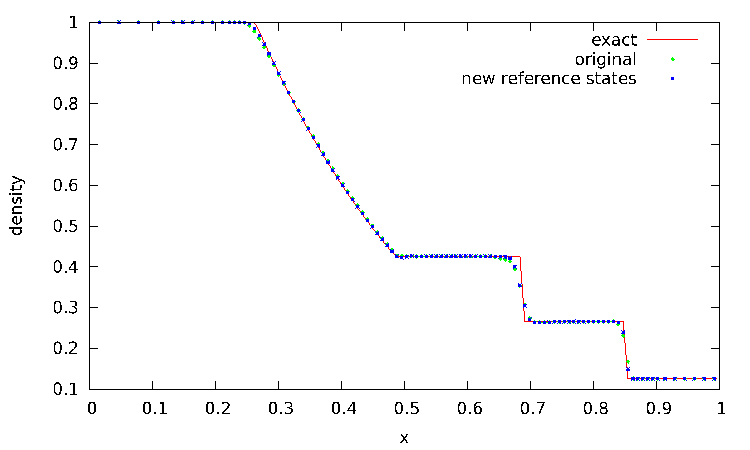
\includegraphics[scale=1.0]{reference}
  \caption{ \label{Fig:sod} Solution to Sod's problem with the original
    reference state and the new reference state, as compared to the
    exact solution.  We note that the new reference state shows a
    slightly sharper shock and contact, but also has a dip at the tail
    of the rarefaction.}
\end{figure}

\clearpage

\begin{figure}
  \centering
  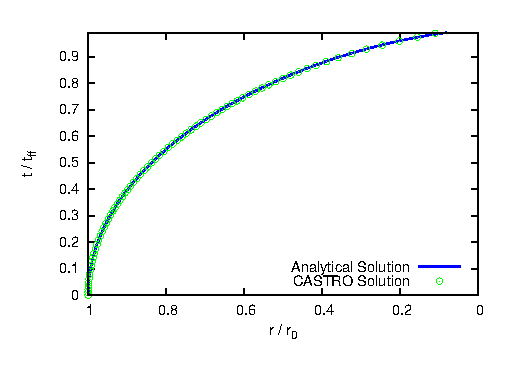
\includegraphics[scale=2.0]{freefall/plot_freefall}
  \caption{Time evolution of two initially stationary white dwarfs,
    mutually attracted to each other by the gravitational force. The
    horizontal axis gives the separation of the white dwarfs, scaled
    to the initial separation, and the vertical axis gives the elapsed
    time of the simulation, scaled to the total elapsed time
    necessarily. The solid curve shows the analytical result,
    calculated from Newtonian mechanics, and the circles show the
    samples from the time evolution with CASTRO. The agreement between
    theory and simulation is excellent, even for a simulation with
    modest resolution.}
  \label{Fig:Free Fall}
\end{figure}


\end{document}

